The last chapter introduced some fundamental topics related to image processing, namely filtering, feature detection, and feature description. While these techniques are quite useful for a large number of computer vision applications, they may not be sufficient to extract higher-level information from images. For example, the features that were discussed are \textit{local features} that describe important keypoints of the image, but these may be too localized to discuss higher-level features or semantic content. In some cases it may be possible to correlate local features to extract higher-level information (e.g. image matching), but in other cases higher-level algorithms may be useful (e.g. identifying a particular object in a scene, such as a person). In particular, object recognition is a very important task in robotics and therefore some common methods for object recognition will be discussed in this chapter.

This chapter will additionally focus on geometric feature extraction\cite{SiegwartNourbakhshEtAl2011}, which is used to extract structure from data in the form of geometric primitives (e.g. lines, circles, planes). This is very useful in robotics for localization and mapping, and these algorithms can generally be applied to different types of data, such as data extracted from images or even data collected via laser rangefinders or radar.

\notessection{Information Extraction}
This chapter will focus on common methods for extracting higher-level environmental information from sensor data that is useful for robotics. In particular, common algorithms for \textit{geometric feature extraction} will be presented, as well as methods for \textit{object recognition} in images. Such information is crucial for robots operating in real environments to enable intelligent decision making and task planning, as well as to execute plans safely in unknown environments with obstacles.

\subsection{Geometric Feature Extraction}
It is very common in robotic localization and mapping to represent the environment using simple geometric primitives (e.g. lines, circles, corners, planes) that can be efficiently extracted from sensor data. In particular, in this section techniques for line extraction from range data\footnote{Range data can generally come from a variety of sources, including laser rangefinders, radar, or even computer vision.} will be presented. Lines in particular are one of the most fundamental geometric primitives to be extracted, and generally the techniques for extracting other primitives are conceptually similar.

There are two main challenges with extracting lines from range data. The first is called \textit{segmentation}, which is the task of identifying which data points belong to which line (and inherently also identifying how many lines there are). The second is \textit{fitting}, which is the task of estimating the parameters that define a line given a set of points. For simplicity this chapter will consider line extraction problems based on two-dimensional range data.

\subsubsection{Line Segmentation}
The line segmentation problem is to determine how many lines exist in a given set of data and also which data points correspond to each line. Three popular algorithms for line segmentation will be discussed, the \textit{split-and-merge} algorithm, the \textit{random sample consensus (RANSAC)} algorithm, and the \textit{Hough-transform} algorithm.




\paragraph{Split-and-Merge:}
The split-and-merge algorithm is perhaps the most popular line extraction algorithm and is arguably the fastest (but not as robust to outliers). The concept of this algorithm is quite simple: repeatedly fit lines to sets of points and then split the set of points into two sets if any point lies more than distance $d$ from the line. By repeating this process until no more splits occur, it is guaranteed that all points will lie less than distance $d$ to a line. After this ``split'' process is completed, a second step merges any of the newly formed lines that are colinear. This algorithm is presented in more detail in Algorithm \ref{alg:splitmerge}.
\begin{algorithm}[ht]\caption{Split-and-Merge} \label{alg:splitmerge}
	\KwData{Set $S$ of $N$ points, distance threshold $d > 0$}
	\KwResult{A list $L$ of sets of points each resembling a line}
	$L \xleftarrow{} [S]$ \\
	$i \xleftarrow{} 1$ \\
	\While{$i \leq \text{len}(L)$}{
	    fit a line $(\alpha,r)$ to the set $L[i]$ \\
	    detect the point $P \in L[i]$ with maximum distance $D$ to the line $(\alpha, r)$ \\
	    \eIf{$D < d$}{
	        $i \xleftarrow{} i + 1$
	    }
	    {
	    split $L[i]$ at $P$ into new sets $S_1$ and $S_2$ \\
	    $L[i] \xleftarrow{} S_1$ \\
	    $L[i+1] \xleftarrow{} S_2$ \\
	    }
	}
	Merge colinear sets in $L$
\end{algorithm}
A popular variant of the split-and-merge algorithm is known as the iterative-end-point-fit algorithm. This algorithm is simply the split-and-merge algorithm given in Algorithm \ref{alg:splitmerge} where the line is simply constructed by connecting the first and the last points of the set. This approach is shown graphically in Figure \ref{fig:splitmerge}.
\begin{figure*}[ht]
\centering
	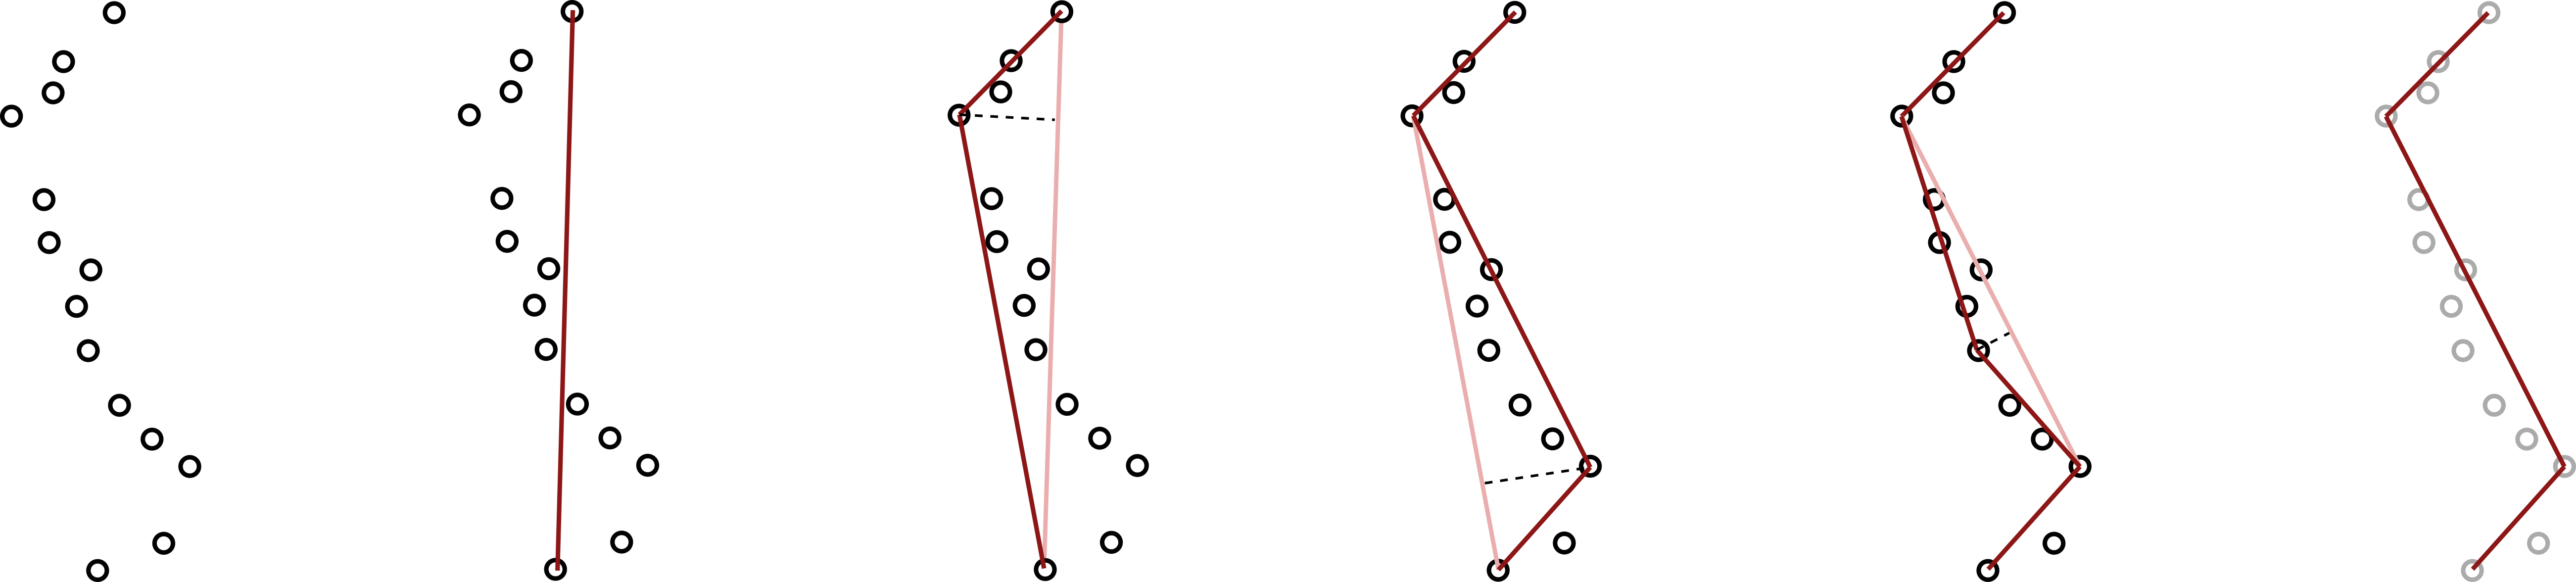
\includegraphics[width=0.85\textwidth]{tex/figs/ch12_fig/iterative_end_point_fit.png}
	\caption{Iterative-end-point-fit variation of the split-and-merge algorithm for extracting lines from data.}
	\label{fig:splitmerge}
\end{figure*}

\paragraph{Random Sample Consensus (RANSAC):}
Random Sample Consensus (RANSAC) is an algorithm to estimate the parameters of a model from a set of data that may contain outliers (i.e. \textit{robust} model parameter estimation). Outliers are data points that do not fit the model and may be the result of high noise in the data, incorrect measurements, or simply points which come from objects that are unrelated to the current model. For example, a typical laser scan of an indoor environment may contain distinct lines from the surrounding walls but also points from other static and dynamic objects (e.g. chairs or humans). In this case, if the goal was to extract lines to represent the walls then any data point corresponding to other objects would be an outlier. In general, RANSAC can be applied to many parameter estimation problems, and typical applications in robotics include line extraction from 2D range data, plane extraction from 3D point clouds, and structure-from-motion (where the goal is to identify image correspondences which satisfy a rigid body transformation). However for simplicity this section focuses on using RANSAC for line extraction from 2D data.

RANSAC is an iterative method and is non-deterministic (i.e. stochastic or random). 
Given a dataset $S$ of $N$ points, the algorithm starts by randomly selecting a sample of two points from $S$. Then a line is constructed from these two points and the distance of all other points to this line is computed. A set of \textit{inliers} comprised of all the points whose distance to the line is within a predefined threshold $d$ is then defined. By repeating this process $k$ times, $k$ inlier sets (and their associated lines) are generated and the inlier set with the most points is returned. This procedure is detailed in Algorithm \ref{alg:ransac} and is also illustrated in Figure \ref{fig:ransac-working}.
\begin{algorithm}[ht]\caption{Random Sample Consensus (RANSAC) for Line Extraction} \label{alg:ransac}
	\KwData{Set $S$ of $N$ points, distance threshold $d$}
	\KwResult{Set with maximum number of inliers and corresponding line}
	\While{$i \leq k$}{
	    randomly select 2 points from $S$ \\
	    fit line $l_i$ through the 2 points \\
	    compute distance of all other points to $l_i$ \\
	    construct set of points $\tilde{S}_i$ with distance less than $d$ to $l_i$ \\
	    store line $l_i$ and set of points $\tilde{S}_i$
	    $i \xleftarrow{} i + 1$
	}
	Choose set $\tilde{S}_i$ with maximum number of points
\end{algorithm}

\begin{figure}[ht]
  \centering
  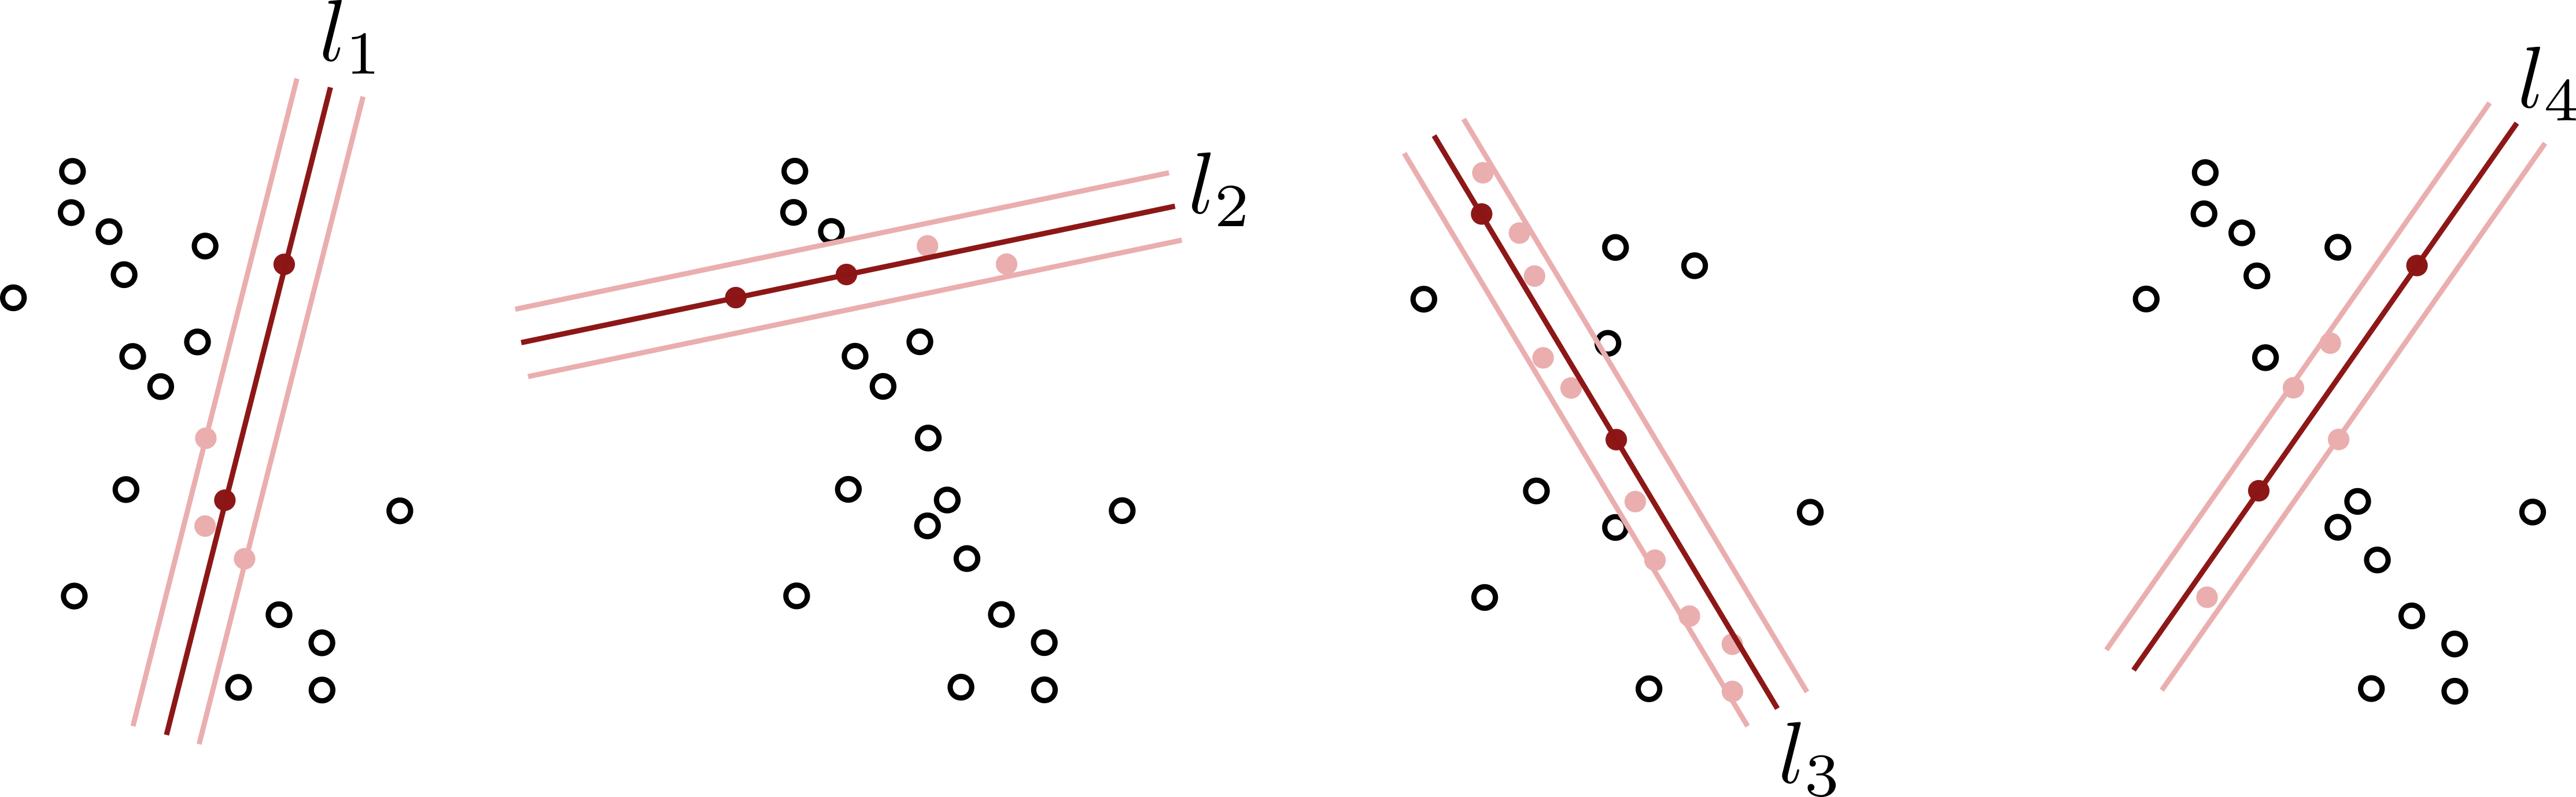
\includegraphics[width=0.85\textwidth]{tex/figs/ch12_fig/ransac.png}
\caption{Example of the RANSAC algorithm, showing four iterations of the algorithm. If the algorithm was terminated after these four iterations, line $l_3$ would be returned since it contains the maximum number of points.}
\label{fig:ransac-working}
\end{figure}

Due to the probabilistic nature of the algorithm, as the number of iterations $k$ increases the probability of finding a good solution increases. This approach is used over a brute force search of all possible combinations of two points since the total number of combinations is $N(N-1)/2$, which can be extremely large. In fact, a simple statistical analysis of RANSAC can be performed.

Let $p$ be the \textit{desired} probability of finding a set of points free of outliers and let $w$ be the probability of selecting an inlier from the dataset $S$ of $N$ points, which can be expressed as:
\begin{equation*}
    w = \frac{\text{\# inliers}}{N}.
\end{equation*}
Assuming point samples are drawn independently from $S$, the probability of drawing two inliers is $w^2$ (and $1-w^2$ is the probability that at least one is an outlier). Therefore, with $k$ iterations the probability that RANSAC \textit{never} selects two points that are both inliers is $(1-w^2)^k$. Therefore the minimum number of iterations $\bar{k}$ needed to find an outlier-free set with probability $p$ can be found by solving:
\begin{equation*}
    1-p = (1-w^2)^k,
\end{equation*}
for $k$. In other words, $\bar{k}$ can be computed as:
\begin{equation*}
    \bar{k} = \frac{\log (1-p)}{\log (1-w^2)}.
    \label{eq:magic-k}
\end{equation*}
While the value of $w$ may not be known exactly\footnote{There also exist advanced versions of RANSAC that can estimate $w$ in an adaptive online fashion.}, this expression can still be used to get a good estimate of the number of iterations $k$ that are needed for good results. It is important to note that this probabilistic approach often leads to a much smaller number of iterations than for brute force searching through all combinations. This can be attributed to the fact that $\bar{k}$ is only a function of $w$ and not the total number of samples $N$ in the dataset. 

Overall, the main advantage of RANSAC is that it is a generic extraction method and can be used with many types of features given a feature \textit{model}. It is also simple to implement and is robust with respect to outliers in the data. The main disadvantages are that the algorithm needs to be run multiple times if multiple features are to be extracted, and there are not guarantees that the solutions will be optimal.

\paragraph{Hough Transform:}
In the Hough transform algorithm, each point $(x_i,y_i)$ of the set $S$ ``votes'' for a \textit{set} of possible line parameters $(m,b)$ (i.e. slope and intercept). For any given point $(x_i,y_i)$ the candidate set of line parameters $(m,b)$ that could pass through this point must satisfy $y_i=mx_i+b$, which can also be written as:
\begin{equation*}
\quad b=-mx_i + y_i.
\end{equation*}
Therefore it can be noted that each point in the original space space $(x,y)$ maps to a \textit{line} in the Hough space $(m,b)$ (see Figure \ref{fig:hough1}). The Hough transform algorithm exploits this fact by noting that two points on the same line in the original space will yield two \textit{intersecting} lines in Hough space. In particular, the point where they intersect in the Hough space corresponds to the parameters $m^*$ and $b^*$ that defines the line passing between the points in the original space (see Figure \ref{fig:hough2}).
\begin{figure}[ht]
  \centering
  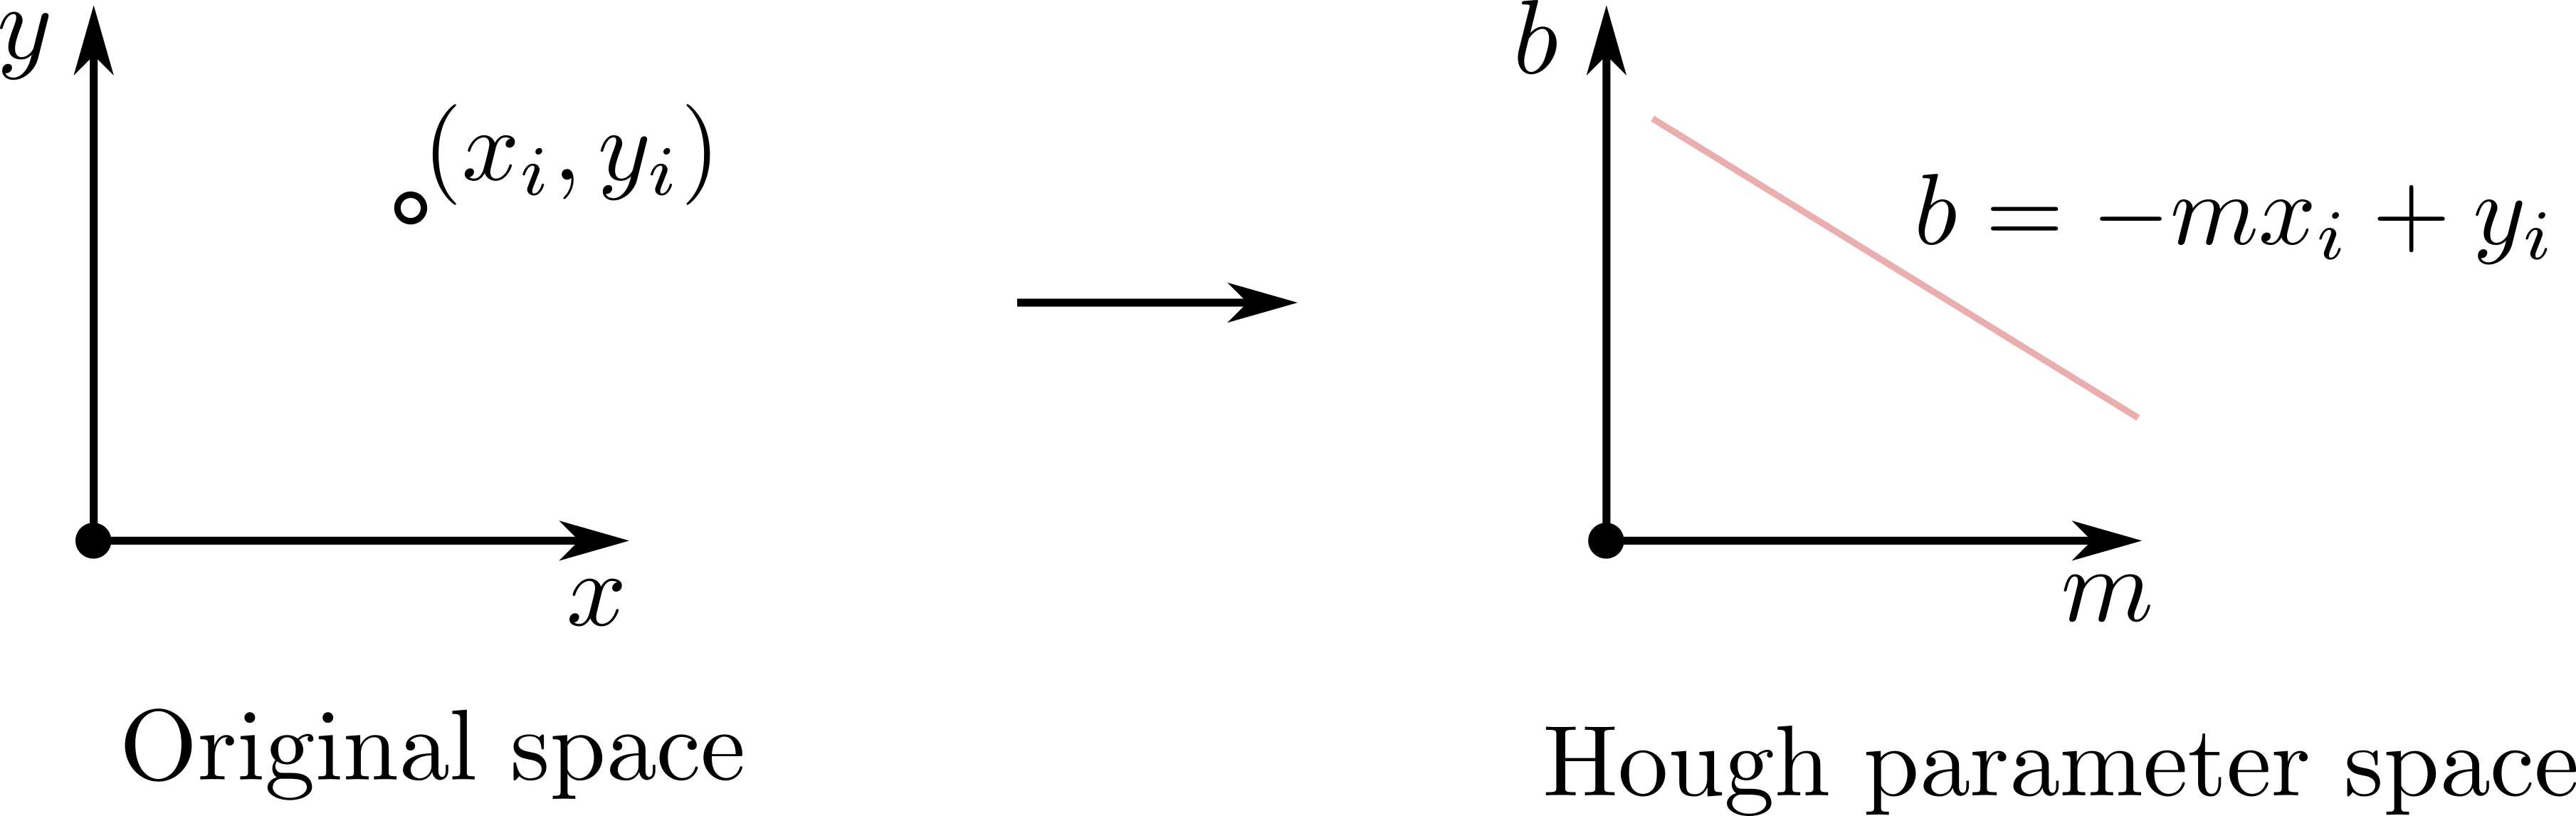
\includegraphics[width=0.75\textwidth]{tex/figs/ch12_fig/hough.png}
\caption{Each point $(x_i, y_i)$ in the original space maps to a \textit{line} in the Hough space which describes all possible parameters $m$ and $b$ that would generate a line passing through the point $(x_i, y_i)$.}
\label{fig:hough1}
\end{figure}
\begin{figure}[ht]
  \centering
  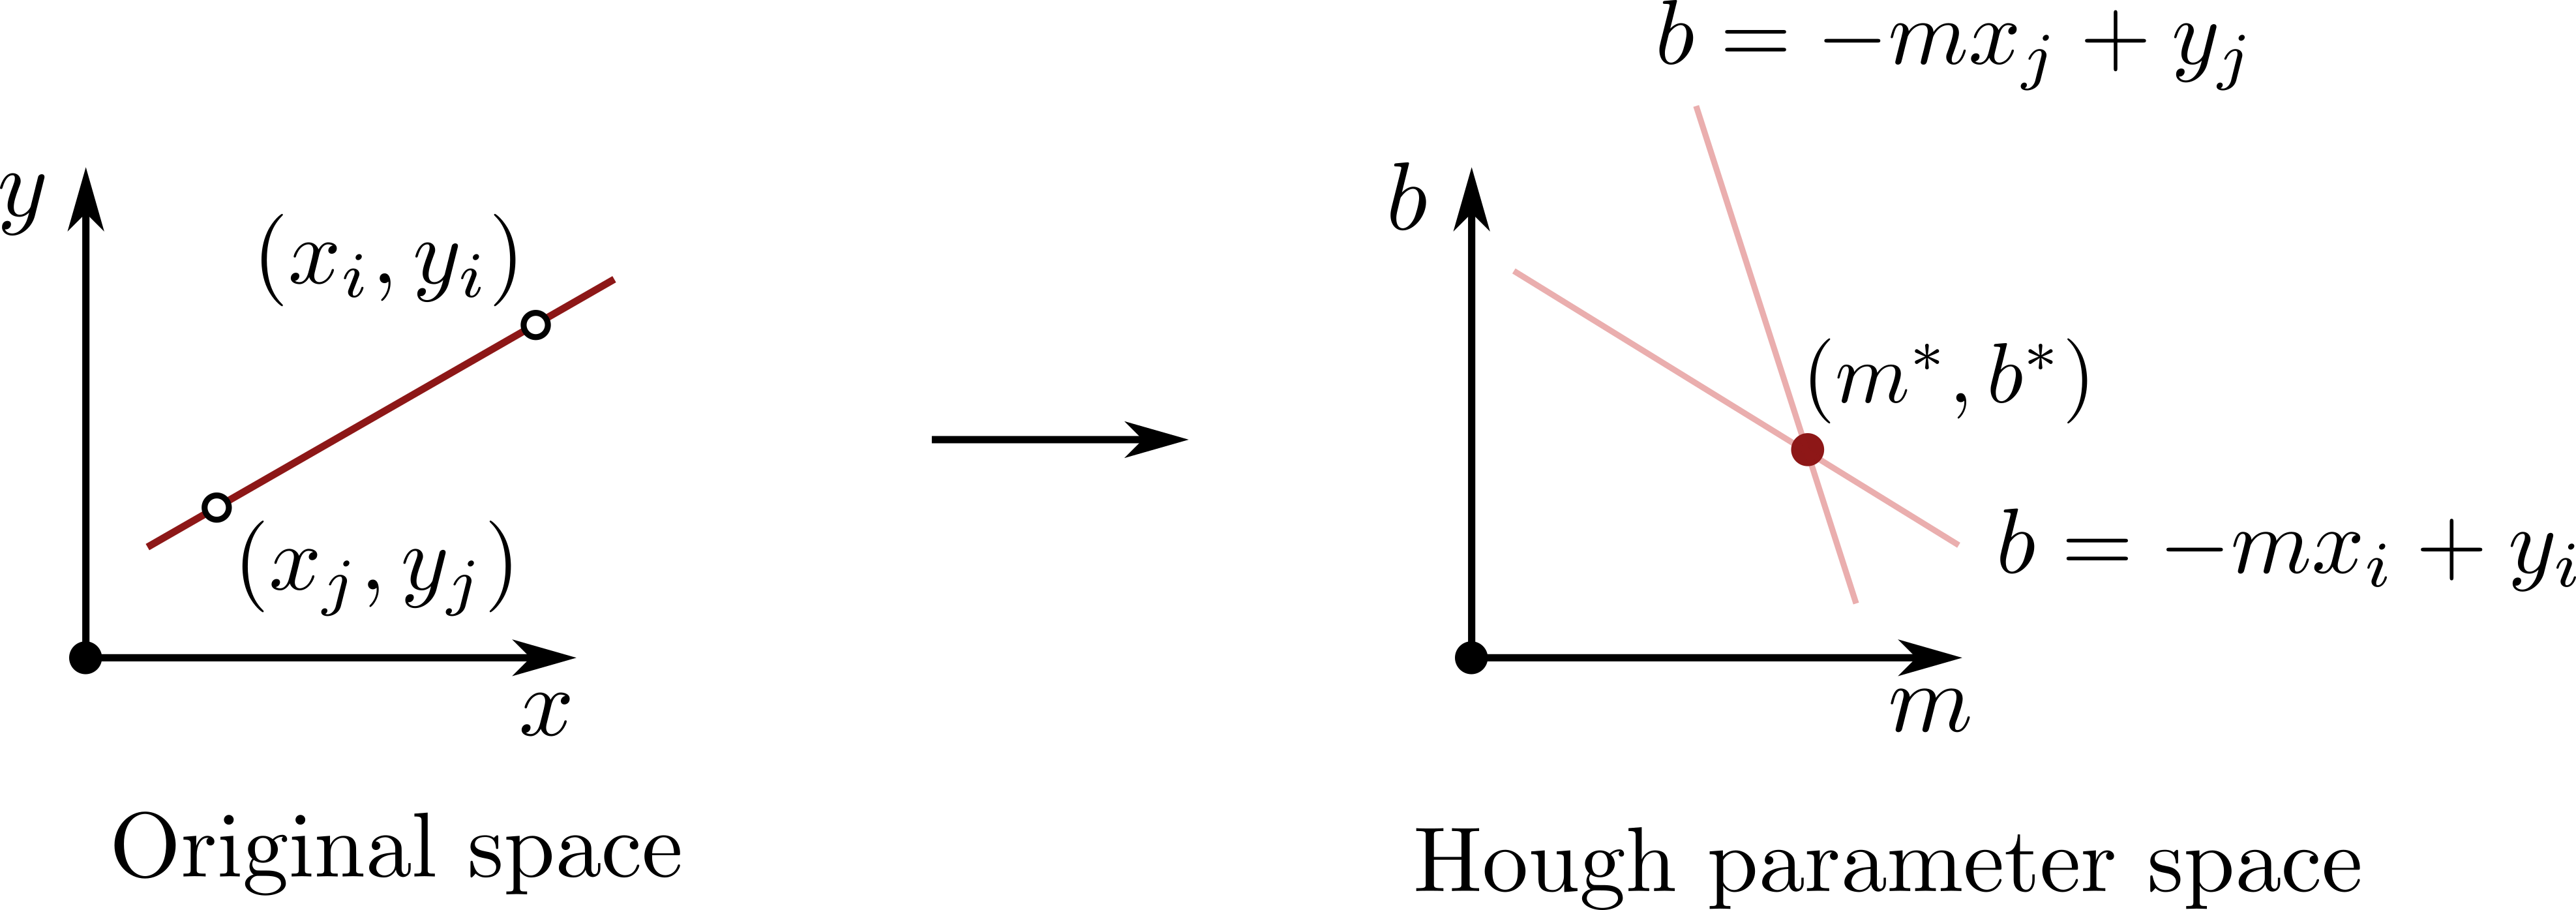
\includegraphics[width=0.75\textwidth]{tex/figs/ch12_fig/hough2.png}
\caption{All points on a line in the original space yield lines in the Hough space that intersect at a common point.}
\label{fig:hough2}
\end{figure}

This concept can be applied to line segmentation by searching in the Hough space for intersections among the lines that correspond to each point $(x,y)$ in the set $S$. In practice, this can be done by discretizing the Hough space with a grid and simply counting for each grid cell the number of lines corresponding to $(x_i,y_i)$ points from $S$ that pass through it. Local maxima among the cells then can be chosen as lines that ``fit'' the data set $S$.

However, performing a discretization of the Hough space requires a trade-off between range and resolution (in particular because $m$ can range from $-\infty$ to $\infty$. Alternatively, it is possible to use a polar coordinate representation of the Hough space which defines a line as:
\begin{equation*}
x \cos \alpha + y \sin \alpha = r,
\end{equation*}
where $(\alpha,r)$ are the new line parameters. With this representation, a point $(x_i,y_i)$ from the original space gets mapped to the polar Hough space $(\alpha,r)$ as a sinusoidal curve (see Figure \ref{fig:hough3}). An example of the Hough transform using the polar representation is given in Figure \ref{fig:hough4}.
\begin{figure}
\centering
	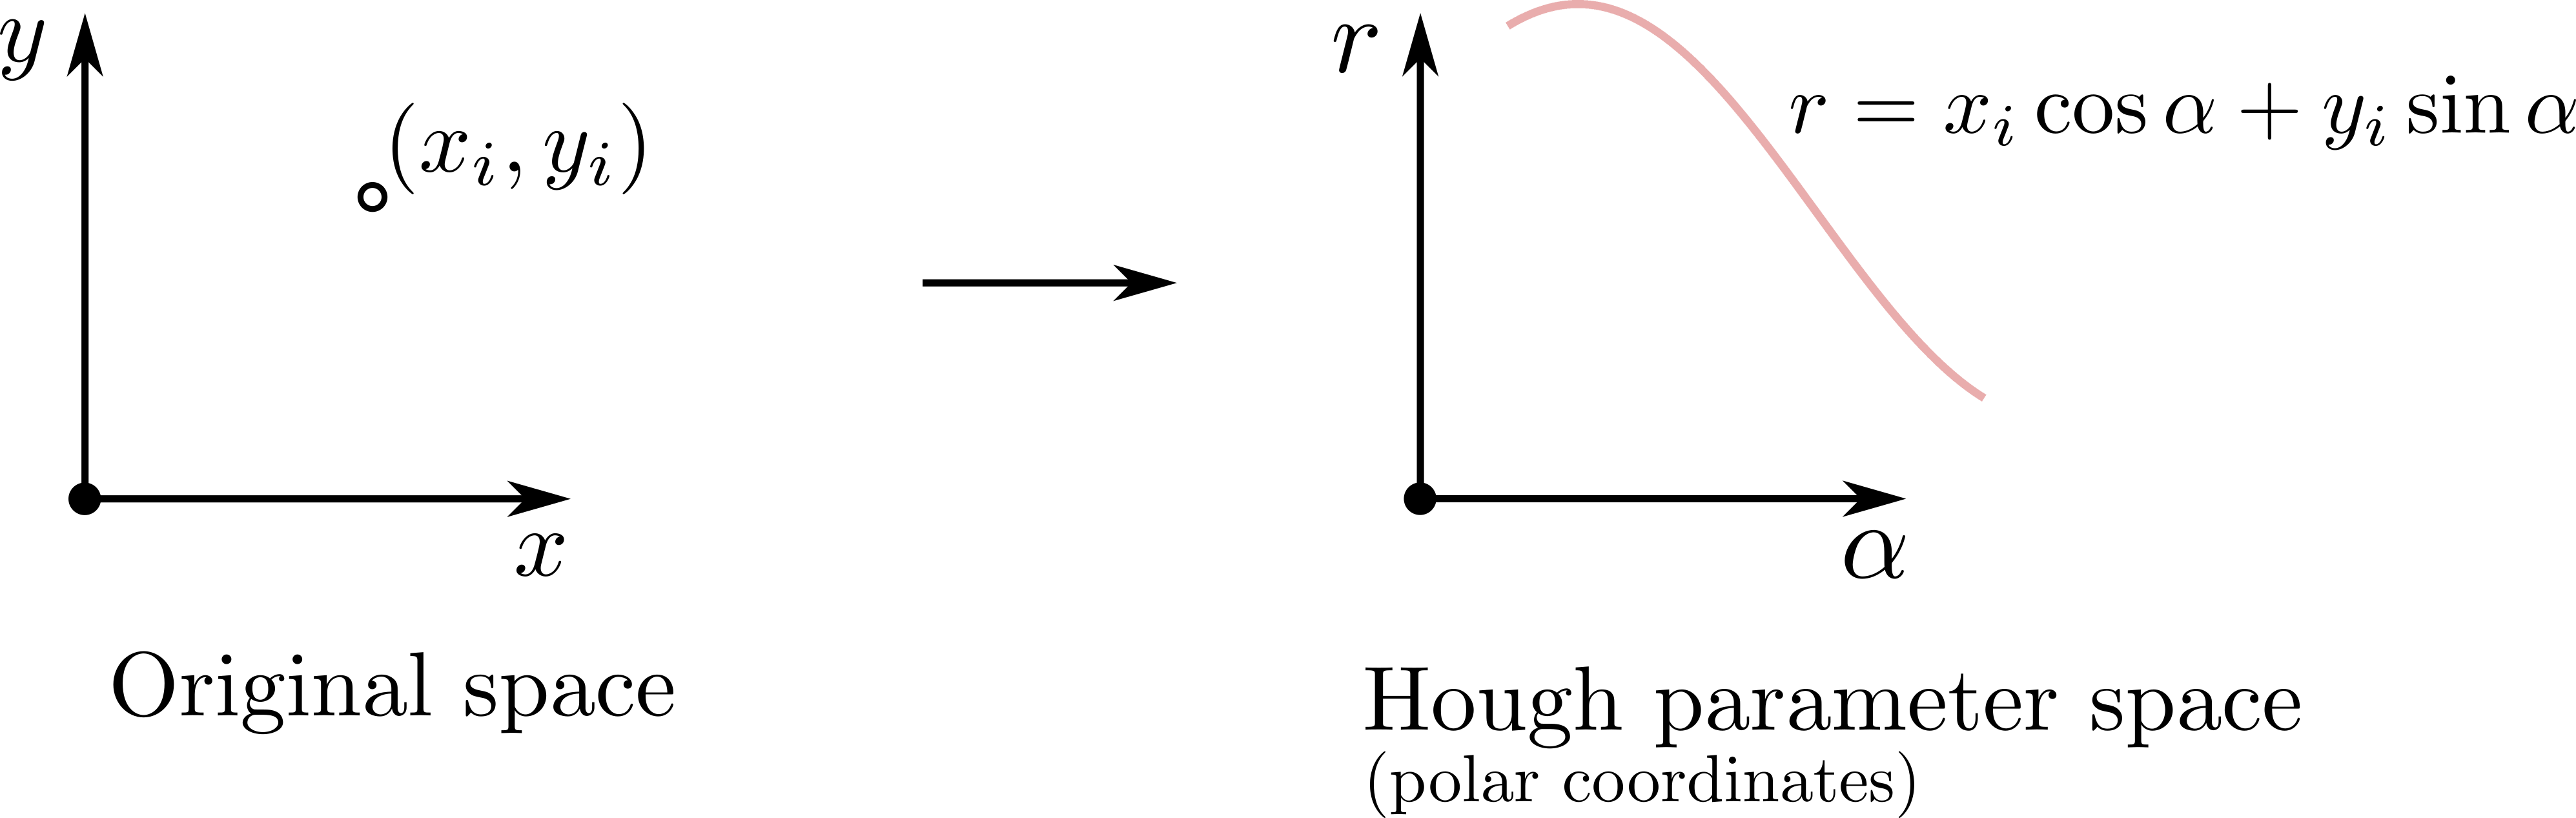
\includegraphics[width=0.75\textwidth]{tex/figs/ch12_fig/hough3.png}
	\caption{Representation of a point $(x_i, y_i)$ in the Hough space when using a polar coordinate representation of a line with parameters $\alpha$ and $r$.}
	\label{fig:hough3}
\end{figure}
\begin{figure}
\centering
	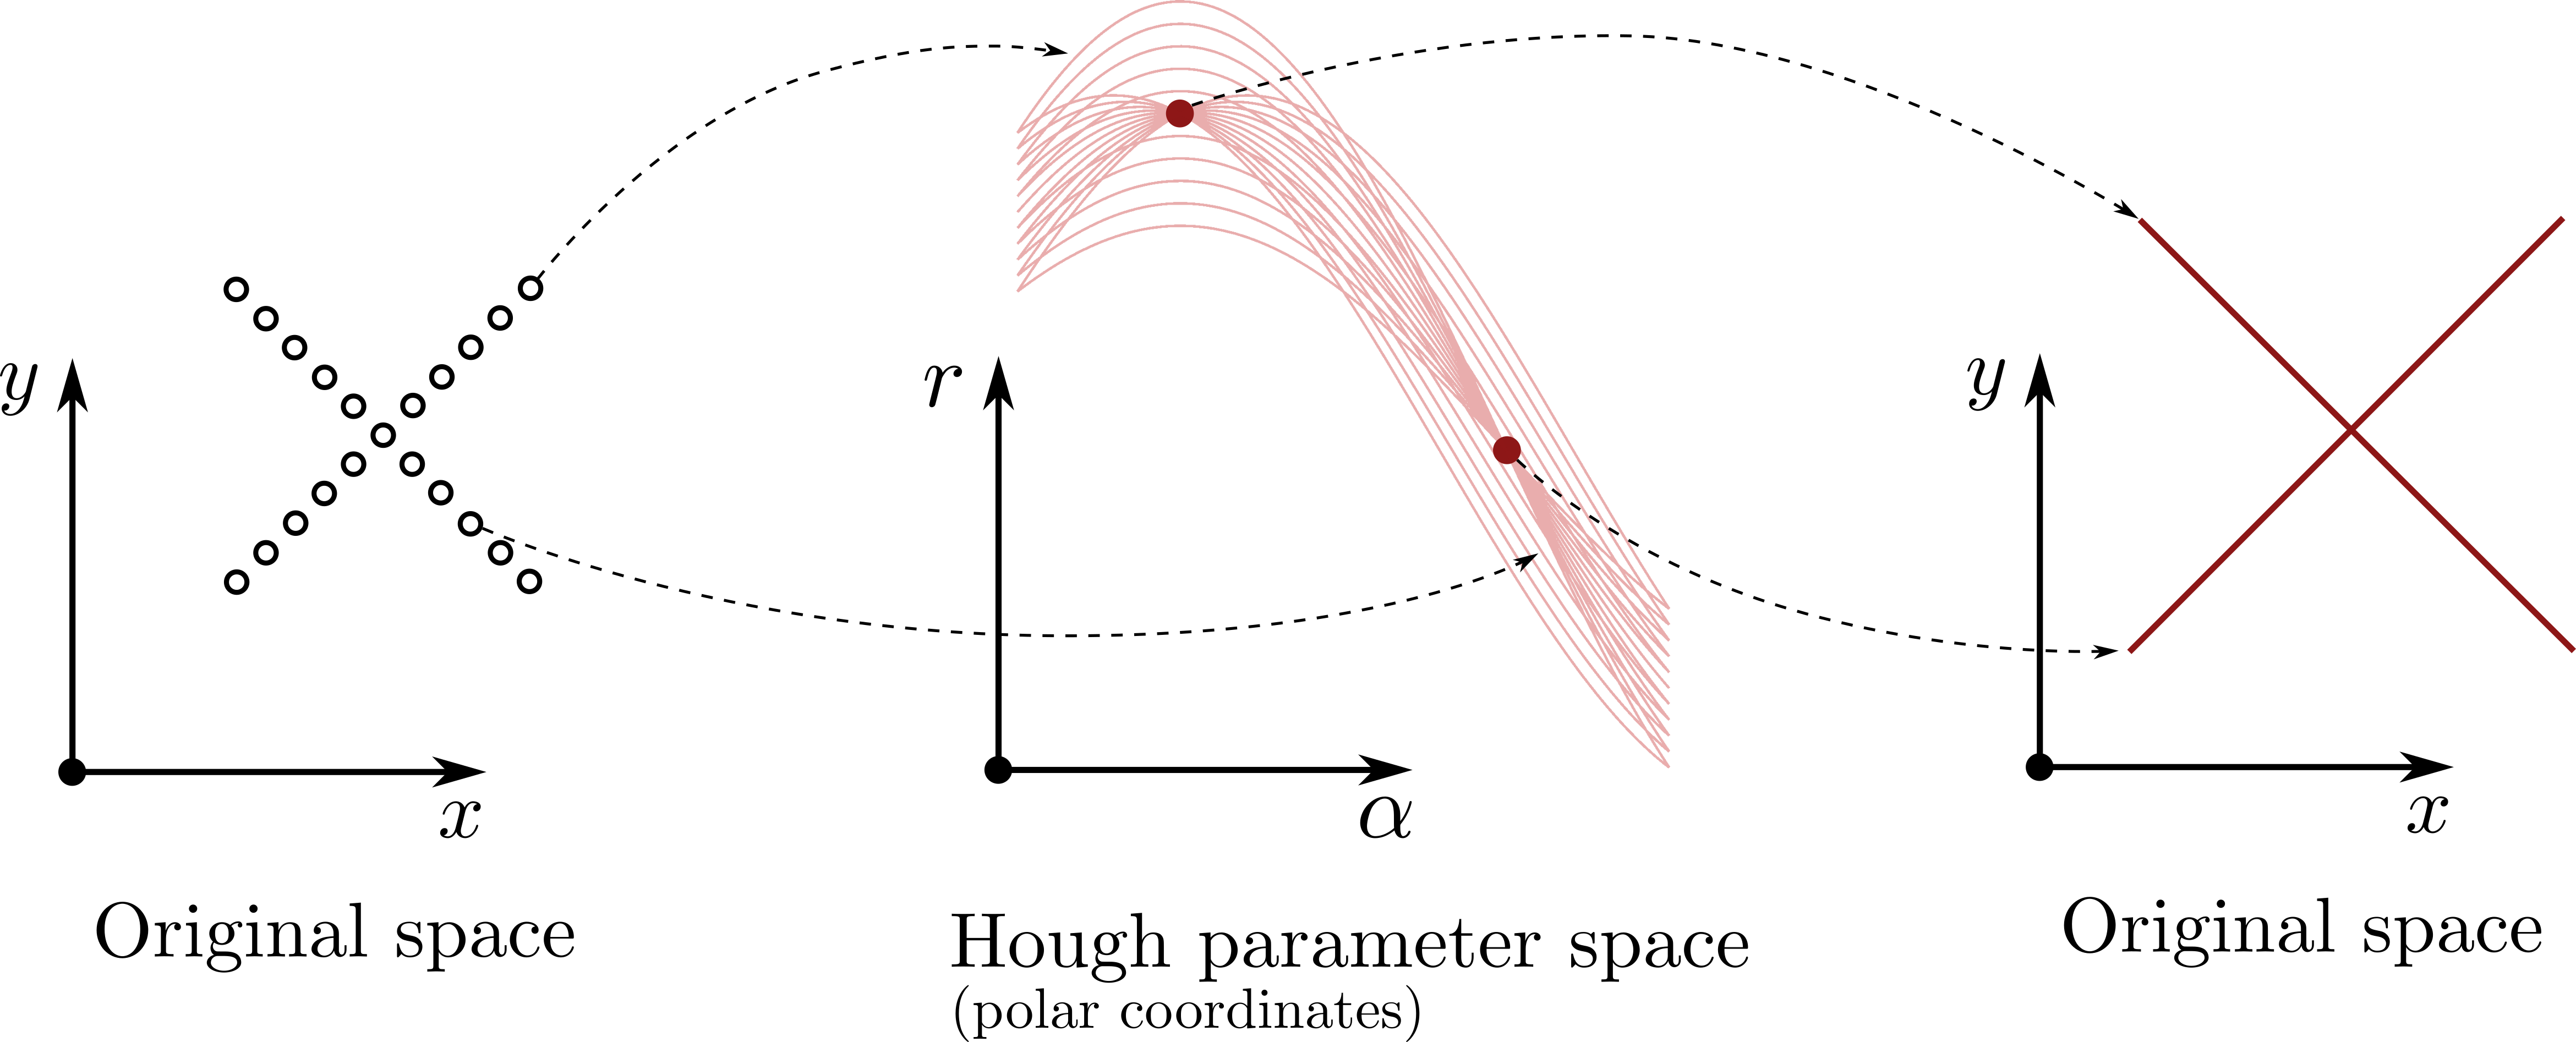
\includegraphics[width=0.85\textwidth]{tex/figs/ch12_fig/hough4.png}
	\caption{Example of the Hough transformation using a polar coordinate representation of lines.}
	\label{fig:hough4}
\end{figure}

\subsubsection{Line Fitting}
Line segmentation is the process of identifying which data points belong to a line, and line fitting is the process of estimating parameters of a line for those corresponding data points. For the line segmentation algorithms previously discussed (i.e. split-and-merge, RANSAC, and Hough-transform), a line associated with the segmented data points was also implicitly defined. However, the lines implicitly defined from the segmentation algorithms may not always be ideal and so other techniques have been developed to specifically address the line fitting task.

Line fitting algorithms search for lines that best fit a set of data points. In almost all cases the problem is over-determined (i.e. there are more data points than parameters to choose) and noise in the data means that there is not perfect solution. Therefore one of the most common approaches to line fitting is based on \textit{least-squares estimation}, which tries to find a line that minimizes the overall error in the fit. For this approach it is useful to work in polar coordinates defined by:
\begin{equation*}
    x = \rho \cos \theta, \quad y = \rho \sin \theta,
\end{equation*}
where $(x,y)$ is the 2D Cartesian coordinate of a data point and $(\rho,\theta)$ is the 2D polar coordinate. In polar coordinates the equation of a line is given by
\begin{equation} \label{eq:polarline}
\rho \cos(\theta - \alpha) = r, \quad \text{or} \quad  x \cos \alpha + y \sin \alpha = r,
\end{equation}
where $\alpha$ and $r$ are the parameters that define the line. For a visual representation of these definitions see Figure \ref{fig:polarline}.
\begin{marginfigure}
  \centering
  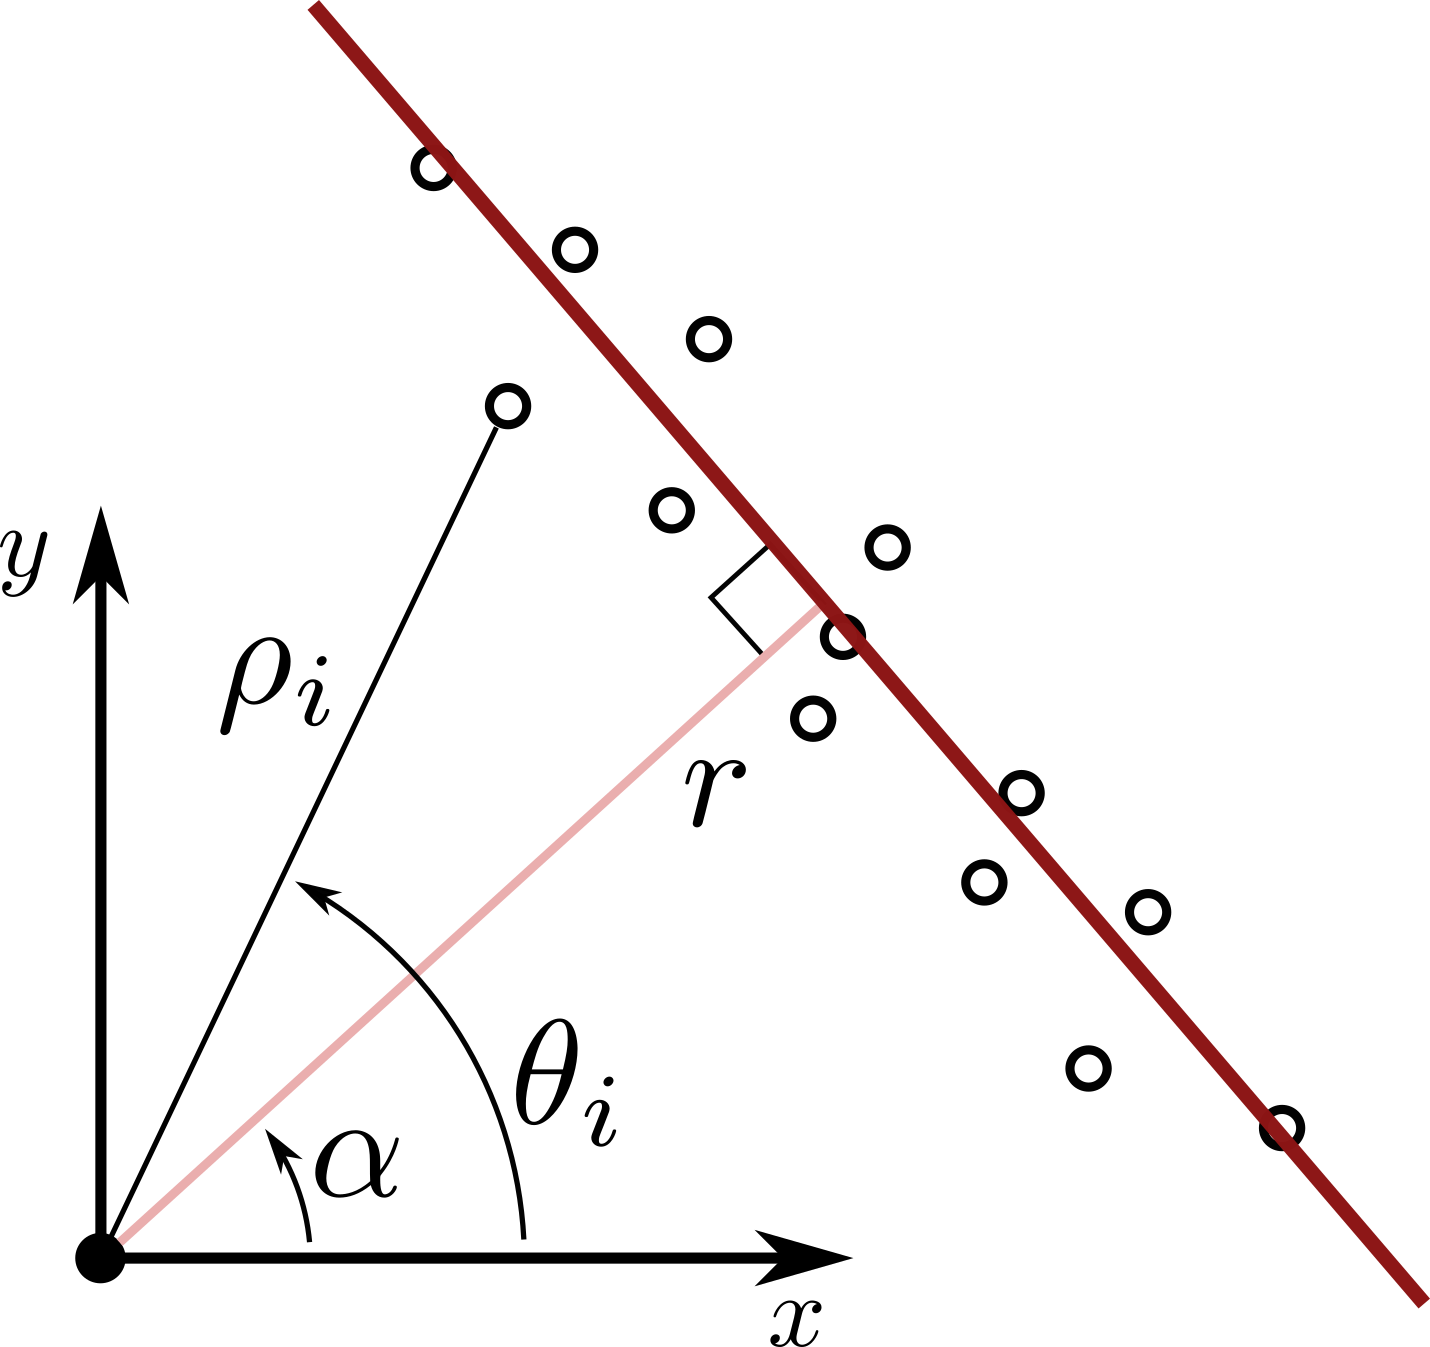
\includegraphics[width=0.85\textwidth]{tex/figs/ch12_fig/polarlinefit.png}
  \caption{Representation of a line in polar coordinates, defined by the parameters $r$ and $\alpha$ which are the distance and angle to the closest point on the line to the origin.}
  \label{fig:polarline}
\end{marginfigure}
For a collection $S$ of $N$ points $(\rho_i, \theta_i)$, the error $d_i$ corresponding to the perpendicular distance from a point to a line defined by parameters $\alpha$ and $r$ can be computed by:
\begin{equation} \label{eq:lineerror}
d_i = \rho_i \cos(\theta_i - \alpha) - r.
\end{equation}
The line fitting task can then be formulated as an optimization problem over the parameters $\alpha$ and $r$ to minimize the combined errors $d_i$ for $i = 1,\dots,N$. In particular, the combined errors are aggregated using a sum of the squared errors:
\begin{equation}
    S(r,\alpha) = \sum_{i=1}^N d_i^2 = \sum_{i=1}^N(\rho_i \cos(\theta_i - \alpha) - r)^2.
    \label{eq:MSL}
\end{equation}
This is a classic least squares optimization problem that can be efficiently solved. However, this cost function generally assumes that each of the data points is equally affected by noise (i.e. the uncertainty of each measurement is the same). In some cases it might be beneficial to account for differences in data quality for each point $i$, which could give preference to well known points.

Accounting for unique uncertainties in each data point leads to a \textit{weighted least squares estimation} problem. In particular, it is assumed that the variance of each range measurement $\rho_i$ is given by $\sigma_i$. The cost function \eqref{eq:MSL} is then modified to be: 
\begin{equation} \label{eq:WMSL}
    S_w(r,\alpha) = \sum_{i=1}^N w_i d_i^2 = \sum_{i=1}^N w_i (\rho_i \cos (\theta_i -\alpha) -r)^2,
\end{equation}
where the weights $w_i$ are given by:
\begin{equation*}
    w_i = \frac{1}{\sigma^2_i}.
\end{equation*}
It can be shown that the solution to the optimization problem defined by the weighted cost function \eqref{eq:WMSL} is given by:
\begin{equation}
\begin{split}
r &= \frac{\sum_{i=1}^N w_i\rho_i\cos(\theta_i - \alpha)}{\sum_{i=1}^N w_i}, \\
\alpha &= \frac{1}{2} \text{atan2} \left(\frac{\sum_{i=1}^N w_i\rho_i^2\sin(2\theta_i) - \frac{2}{\sum_{i=1}^N w_i}\sum_{i=1}^N\sum_{j=1}^N w_i w_j \rho_i \rho_j \cos\theta_i \sin \theta_j}{\sum_{i=1}^N w_i \rho_i^2\cos(2\theta_i) - \frac{1}{\sum_{i=1}^N w_i}\sum_{i=1}^N\sum_{j=1}^N w_i w_j \rho_i \rho_j \cos(\theta_i + \theta_j)}\right) + \frac{\pi}{2}.
\end{split}
\end{equation}

\subsection{Object Recognition}
Another high-level information extraction task that is common in robotics is \textit{object recognition}. Object recognition is the task of classifying or naming discrete objects in the world (usually based on images or video). This can be a particularly challenging task because real world scenes are commonly made up of many varying types of objects which can appear at different poses and can occlude each other. Additionally, objects within a specific class can have a large amount of variability (e.g. breeds of dogs or car models). In this section three common methods for object recognition will be introduced, namely template matching, bag of visual words, and neural network methods.

\subsubsection{Template Matching}
Template matching\cite{PerveenKumarEtAl2013} is a machine vision technique for identifying parts of an image that match a given image pattern\footnote{Advanced template matching algorithms allow finding pattern occurrences regardless of their orientation and local brightness.}. This approach has seen success in a variety of applications, including manufacturing quality control, mobile robotics, and more. The two primary components needed for template matching are the source image $I$ and a template image $T$

Given a source and template image, one approach to template matching is to leverage the linear spatial correlation filters discussed in the previous chapter. In particular, a naive approach would be to use the normalized template image as a filter mask in a correlation filter. By applying this filter mask to every pixel in the source image the resulting output would quantify the similarity of that region of the source image to the template. This type of approach is sometimes referred to as a \textit{cross-correlation}.
Another approach based on linear spatial filters from the previous chapter would be to leverage the similarity filters that compute the sum of absolute differences (SAD) metric for each pixel in the source image. Regions of the source image similar to the template would correspond to low SAD scores.
The disadvantages of these approaches is that do not handle rotations or scale changes, which are quite common in real world applications.

One solution to the scaling issue in correlation filter based template matching is to simply re-scale the source image multiple times and perform template matching on each. This concept, referred to as using \textit{image pyramids}\cite{Szeliski2010}, can also be used to accelerate object search by using a coarser resolution image first to localize the object and then using finer resolution images for actual detection. Building image pyramids can be accomplished in several ways. One naive approach is to simply eliminate some rows and columns of the image. Another approach is to first use a Gaussian smoothing filter to remove high frequency content form the image and \textit{then} subsample the image. The sequence of images resulting from this approach is referred to as a \textit{Gaussian pyramid}.

\begin{figure}[ht]
  \centering
  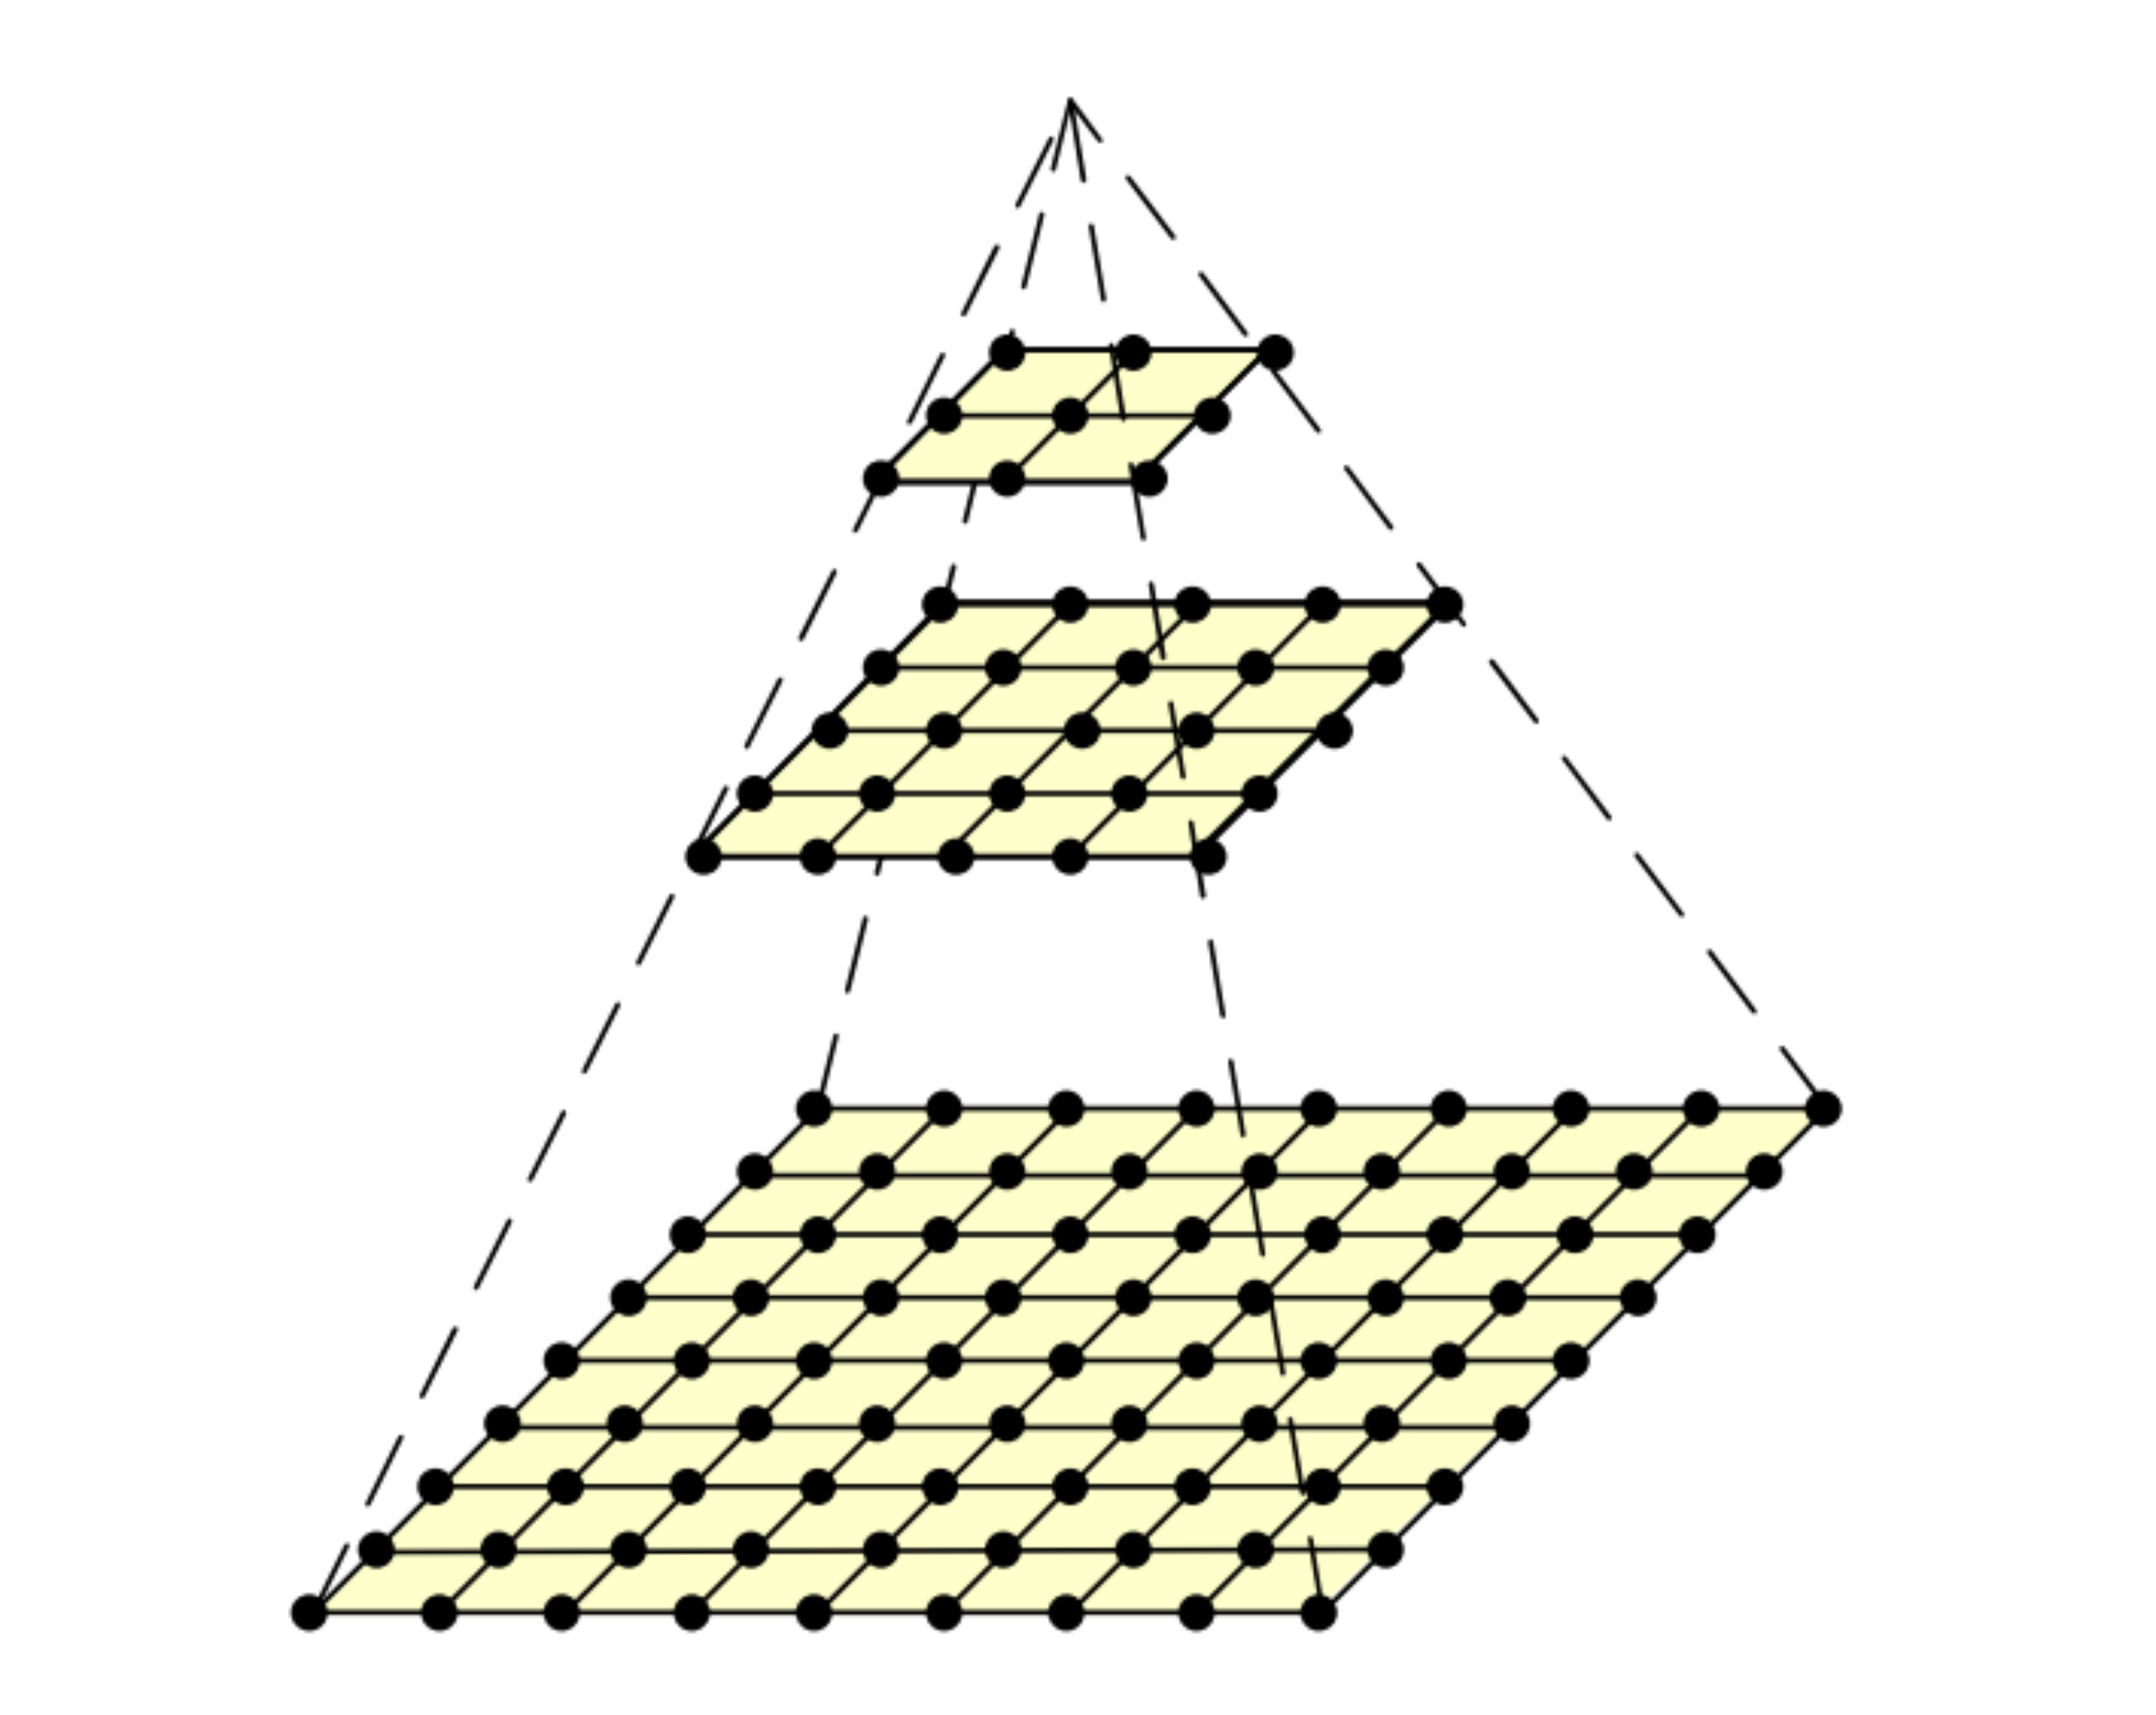
\includegraphics[width=0.6\textwidth]{tex/figs/ch12_fig/image_pyramid.png}
\caption{A traditional image pyramid: each level has half the resolution (width and height), and hence a quarter of the pixels, of its parent level. Figure from Szeliski (2010) \nocite{Szeliski2010}.}
\label{image-pyramid}
\end{figure}

\subsubsection{Bag of Visual Words}
The key idea behind the bag of visual words\footnote{The model originated in natural language processing, where we consider texts such as documents, paragraphs, and sentences as collections of words - effectively ``bags" of words. 
} approach is that object representations can be simplified by considering them as a collection of their subparts (e.g. a bike is an object with wheels, a frame, and handlebars), and the subparts are referred to as \textit{visual words}. In this approach a source image is searched for \textit{visual words}, and a distribution of visual words that are found in the image is created (in the form of a histogram). Object detection can then be performed by comparing this distribution to a set of training images. For example, suppose the source image contains a human face and the recognized features included eyes and a nose. Then by comparing the distribution to training images, it would likely be determined that training images that also have eyes and a nose are also images of faces.

\subsubsection{Convolutional Neural Networks}
Convolutional Neural Networks (CNNs) represent a relatively new and very powerful paradigm in object recognition. These approaches were first introduced in the field of computer vision for image recognition in 1989, and since then have significantly boosted performance in image recognition and classification tasks. Research in this field is also still very active.


\subsection{Exercises}
All exercises for this chapter can be found in the online repository:

\vspace{\baselineskip}

\url{https://github.com/PrinciplesofRobotAutonomy/AA274A_HW3}.

\subsubsection{Line Extraction}
Complete \textit{Problem 2: Line Extraction}, where you will implement a line extraction algorithm (Split-and-Merge) to fit lines to simulated Lidar range data.

\subsubsection{Template Matching}
Complete \textit{Problem 4: Template Matching}, where you will explore the use of the classic template matching algorithm, implemented in the open-source OpenCV library.

\subsubsection{Image Pyramids}
Complete \textit{Extra Problem: Image Pyramids}, where you will learn about how template matching algorithms can be enhanced through the use of image pyramids (and image filtering).